\documentclass[11pt]{article}
\usepackage[utf8]{inputenc}
\usepackage{float}
\usepackage{amsmath}
\usepackage{tikz} % for Hasse diagram
\usepackage[hmargin=3cm,vmargin=6.0cm]{geometry}
%\topmargin=0cm
\topmargin=-2cm
\addtolength{\textheight}{6.5cm}
\addtolength{\textwidth}{2.0cm}
%\setlength{\leftmargin}{-5cm}
\setlength{\oddsidemargin}{0.0cm}
\setlength{\evensidemargin}{0.0cm}

\begin{document}
	
\section*{Student Information } 
%Write your full name and id number between the colon and newline
%Put one empty space character after colon and before newline
Full Name : Beyazıt Yalçınkaya \\
Id Number : 2172138 \\

% Write your answers below the section tags
\section*{Answer 1}

In the question the following properties are given for a graph $G = (V, E)$:
\begin{itemize}
    \item $|E| = 23$
    \item $deg(v) \geq 4, \ for \ all \ v \in V$
\end{itemize}
Since $deg(v) \geq 4, \ for \ all \ v \in V$ is given, the following can be concluded:
\begin{equation*}
    \sum_{v \in V}{deg(v)} \geq 4 \times |V| \\
\end{equation*}
By The Handshaking Theorem the following equation can be derived:
\begin{equation*}
    \begin{split}
        2 \times |E| & = \sum_{v \in V}{deg(v)} \quad (The \ Handshaking \ Theorem) \\
        2 \times |E| & = \sum_{v \in V}{deg(v)} \geq 4 |V| \\
        2 \times |E| & \geq 4 \times |V| \\
        2 \times 23 & \geq 4 \times |V| \\
        46 & \geq 4 \times |V| \\
        11.5 & \geq |V| \\
        Largest \ value & \ of \ |V| \ is \ |V| = 11.
    \end{split}
\end{equation*}
By the equation above $|V|$ must be less than or equal to $11.5$, then the largest value of $|V|$ is $|V| =11$. Thus, the largest possible number of vertices is $11$.


\section*{Answer 2}

Say $G = (V, E)$ is a simple graph with $n$ vertices with $n \geq 2$ such that the degree of every vertex in $G$ is at least $\frac{n - 1}{2}$. Let's add a vertex $v'$ to the graph $G$ and connect it to all other vertices in the graph and name the new graph as $G'$. Since we connected $v'$ with all other vertices, the degree of all other vertices has been incremented by one and note that the degree of $v'$ is $n$. Then the degree of every vertex in $G'$ is at least $\frac{n - 1}{2} + 1$ which is equal to $\frac{n + 1}{2}$. Note that $\frac{n + 1}{2} > \frac{n}{2}$ and $n \geq 3$, then by the Dirac's Theorem, $G'$ has a Hamiltonian circuit. Let's denote this Hamiltonian circuit as a sequence of vertices as follows:
\begin{equation*}
    v_1v_2v_3v_4........v_{n - 1}v_{n}v'v_1\\
\end{equation*}
Now, let's remove the vertex $v'$ and all edges incident to it from $G'$. Note that after this removal the initial graph $G$ has been obtained. The Hamiltonian circuit denoted as a sequence of vertices is no longer valid since the vertex $v'$ is not in $G$. However, all other vertices and the edges connecting them are in the graph since the removing operation of $v'$ and edges incident to it did not affect other vertices and edges. Then the sequence of vertices written above changed as follows:
\begin{equation*}
    v_1v_2v_3v_4........v_{n - 1}v_{n}\\
\end{equation*}
It can be observed that the sequence of vertices above is a Hamiltonian path since all vertices of $G$ is visited exactly once by the path. Note that, for $n = 1$ case, since $G$ contains only $1$ vertex, trivially it has a Hamiltonian path. Thus, a simple graph $G = (V, E)$ with $n$ vertices such that the degree of every vertex in $G$ is at least $\frac{n - 1}{2}$ contains a Hamiltonian path.


\section*{Answer 3}

Say $G = (V, E)$ is a bipartite graph with adjacency matrix $A^{37}$, then $|V| = 37$. Since $G$ is a bipartite graph, its vertices can be partitioned into two disjoint sets $V_1$ and $V_2$ such that every edge in the graph connects a vertex in $V_1$ and a vertex in $V_2$. Assume that there exists a vertex $v_k \in V = \{v_1,v_2,...,v_{36},v_{37}\}$ and an edge $e_k \in E$ such that $e_k$ connects $v_k$ with itself. This implies in the adjacency matrix $A^{37}$, the entry $A^{37}_{kk}$ is $1$. Since an edge in a bipartite graph must connect a vertex in $V_1$ and a vertex in $V_2$, $v_k$ must be in both of the partition sets $V_1$ and $V_2$. However, partition sets $V_1$ and $V_2$ are disjoint sets, so there cannot be a vertex which is in both sets. Thus, this is a contradiction, assumption is discharged, there does not exists a vertex $v_k \in V$ and an edge $e_k \in E$ such that $e_k$ connects $v_k$ with itself, so the entry $A^{37}_{kk}$ is not $1$. Note that $A^{37}_{kk}$ is on the diagonal of $A^{37}$ for all values of $k$, this implies in the adjacency matrix $1$ cannot appear on the diagonal of the matrix. Hence, the diagonal entries of $A^{37}$ are equal to $0$.


\section*{Answer 4}
\begin{itemize}
	\item[\textbf{a.}] ~
        \begin{table}[H]
        \centering
        \label{my-label1}
        \begin{tabular}{c|c|c}
	         Choice & Edge & Weight \\
	         \hline
	         1 & \{e, f\} & 1 \\
	         2 & \{a, d\} & 2 \\
	         3 & \{e, h\} & 2 \\
	         4 & \{g, h\} & 2 \\
	         5 & \{g, d\} & 3 \\
	         6 & \{c, f\} & 3 \\
	         7 & \{d, b\} & 3 \\
	         8 & \{h, i\} & 4 \\
        \end{tabular}
        \end{table}
	\item[\textbf{b.}] ~
        \begin{table}[H]
        \centering
        \label{my-label2}
        \begin{tabular}{c|c|c}
	         Choice & Edge & Weight \\
	         \hline
	         1 & \{e, f\} & 1 \\
	         2 & \{e, h\} & 2 \\
	         3 & \{g, h\} & 2 \\
	         4 & \{g, d\} & 3 \\
	         5 & \{a, d\} & 2 \\
	         6 & \{c, f\} & 3 \\
	         7 & \{d, b\} & 3 \\
	         8 & \{h, i\} & 4 \\
        \end{tabular}
        \end{table}
\end{itemize}

\begin{figure}[H]	\caption{Obtained MST in both part \textbf{a.} and part \textbf{b.}}
	\centering
	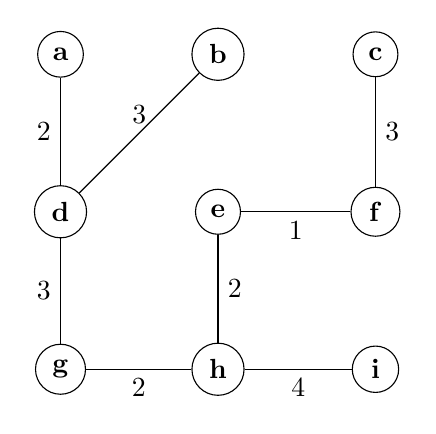
\begin{tikzpicture}
	
	\node[shape=circle,draw=black] (a) at (0, 4)     {\textbf{a}};
	\node[shape=circle,draw=black] (b) at (2, 4)     {\textbf{b}};
	\node[shape=circle,draw=black] (c) at (4, 4)     {\textbf{c}};
	\node[shape=circle,draw=black] (d) at (0, 2)     {\textbf{d}};
	\node[shape=circle,draw=black] (e) at (2, 2)     {\textbf{e}};
	\node[shape=circle,draw=black] (f) at (4, 2)     {\textbf{f}};
	\node[shape=circle,draw=black] (g) at (0, 0)     {\textbf{g}};
	\node[shape=circle,draw=black] (h) at (2, 0)     {\textbf{h}};
	\node[shape=circle,draw=black] (i) at (4, 0)     {\textbf{i}};
	

	\path[-] (a) edge  node[left]  {2} (d);
	\path[-] (b) edge  node[above] {3} (d);



	\path[-] (c) edge  node[right] {3} (f);


	\path[-] (d) edge  node[left]  {3} (g);
	\path[-] (e) edge  node[right] {2} (h);
	\path[-] (e) edge  node[below] {1} (f);


	\path[-] (g) edge  node[below] {2} (h);
	\path[-] (h) edge  node[below] {4} (i);
	
	\end{tikzpicture} 
\end{figure}

\end{document}